% Options for packages loaded elsewhere
\PassOptionsToPackage{unicode}{hyperref}
\PassOptionsToPackage{hyphens}{url}
%
\documentclass[
]{article}
\usepackage{lmodern}
\usepackage{amssymb,amsmath}
\usepackage{ifxetex,ifluatex}
\ifnum 0\ifxetex 1\fi\ifluatex 1\fi=0 % if pdftex
  \usepackage[T1]{fontenc}
  \usepackage[utf8]{inputenc}
  \usepackage{textcomp} % provide euro and other symbols
\else % if luatex or xetex
  \usepackage{unicode-math}
  \defaultfontfeatures{Scale=MatchLowercase}
  \defaultfontfeatures[\rmfamily]{Ligatures=TeX,Scale=1}
\fi
% Use upquote if available, for straight quotes in verbatim environments
\IfFileExists{upquote.sty}{\usepackage{upquote}}{}
\IfFileExists{microtype.sty}{% use microtype if available
  \usepackage[]{microtype}
  \UseMicrotypeSet[protrusion]{basicmath} % disable protrusion for tt fonts
}{}
\makeatletter
\@ifundefined{KOMAClassName}{% if non-KOMA class
  \IfFileExists{parskip.sty}{%
    \usepackage{parskip}
  }{% else
    \setlength{\parindent}{0pt}
    \setlength{\parskip}{6pt plus 2pt minus 1pt}}
}{% if KOMA class
  \KOMAoptions{parskip=half}}
\makeatother
\usepackage{xcolor}
\IfFileExists{xurl.sty}{\usepackage{xurl}}{} % add URL line breaks if available
\IfFileExists{bookmark.sty}{\usepackage{bookmark}}{\usepackage{hyperref}}
\hypersetup{
  pdftitle={Report Title},
  pdfauthor={Student Number},
  hidelinks,
  pdfcreator={LaTeX via pandoc}}
\urlstyle{same} % disable monospaced font for URLs
\usepackage[margin=1in]{geometry}
\usepackage{color}
\usepackage{fancyvrb}
\newcommand{\VerbBar}{|}
\newcommand{\VERB}{\Verb[commandchars=\\\{\}]}
\DefineVerbatimEnvironment{Highlighting}{Verbatim}{commandchars=\\\{\}}
% Add ',fontsize=\small' for more characters per line
\usepackage{framed}
\definecolor{shadecolor}{RGB}{248,248,248}
\newenvironment{Shaded}{\begin{snugshade}}{\end{snugshade}}
\newcommand{\AlertTok}[1]{\textcolor[rgb]{0.94,0.16,0.16}{#1}}
\newcommand{\AnnotationTok}[1]{\textcolor[rgb]{0.56,0.35,0.01}{\textbf{\textit{#1}}}}
\newcommand{\AttributeTok}[1]{\textcolor[rgb]{0.77,0.63,0.00}{#1}}
\newcommand{\BaseNTok}[1]{\textcolor[rgb]{0.00,0.00,0.81}{#1}}
\newcommand{\BuiltInTok}[1]{#1}
\newcommand{\CharTok}[1]{\textcolor[rgb]{0.31,0.60,0.02}{#1}}
\newcommand{\CommentTok}[1]{\textcolor[rgb]{0.56,0.35,0.01}{\textit{#1}}}
\newcommand{\CommentVarTok}[1]{\textcolor[rgb]{0.56,0.35,0.01}{\textbf{\textit{#1}}}}
\newcommand{\ConstantTok}[1]{\textcolor[rgb]{0.00,0.00,0.00}{#1}}
\newcommand{\ControlFlowTok}[1]{\textcolor[rgb]{0.13,0.29,0.53}{\textbf{#1}}}
\newcommand{\DataTypeTok}[1]{\textcolor[rgb]{0.13,0.29,0.53}{#1}}
\newcommand{\DecValTok}[1]{\textcolor[rgb]{0.00,0.00,0.81}{#1}}
\newcommand{\DocumentationTok}[1]{\textcolor[rgb]{0.56,0.35,0.01}{\textbf{\textit{#1}}}}
\newcommand{\ErrorTok}[1]{\textcolor[rgb]{0.64,0.00,0.00}{\textbf{#1}}}
\newcommand{\ExtensionTok}[1]{#1}
\newcommand{\FloatTok}[1]{\textcolor[rgb]{0.00,0.00,0.81}{#1}}
\newcommand{\FunctionTok}[1]{\textcolor[rgb]{0.00,0.00,0.00}{#1}}
\newcommand{\ImportTok}[1]{#1}
\newcommand{\InformationTok}[1]{\textcolor[rgb]{0.56,0.35,0.01}{\textbf{\textit{#1}}}}
\newcommand{\KeywordTok}[1]{\textcolor[rgb]{0.13,0.29,0.53}{\textbf{#1}}}
\newcommand{\NormalTok}[1]{#1}
\newcommand{\OperatorTok}[1]{\textcolor[rgb]{0.81,0.36,0.00}{\textbf{#1}}}
\newcommand{\OtherTok}[1]{\textcolor[rgb]{0.56,0.35,0.01}{#1}}
\newcommand{\PreprocessorTok}[1]{\textcolor[rgb]{0.56,0.35,0.01}{\textit{#1}}}
\newcommand{\RegionMarkerTok}[1]{#1}
\newcommand{\SpecialCharTok}[1]{\textcolor[rgb]{0.00,0.00,0.00}{#1}}
\newcommand{\SpecialStringTok}[1]{\textcolor[rgb]{0.31,0.60,0.02}{#1}}
\newcommand{\StringTok}[1]{\textcolor[rgb]{0.31,0.60,0.02}{#1}}
\newcommand{\VariableTok}[1]{\textcolor[rgb]{0.00,0.00,0.00}{#1}}
\newcommand{\VerbatimStringTok}[1]{\textcolor[rgb]{0.31,0.60,0.02}{#1}}
\newcommand{\WarningTok}[1]{\textcolor[rgb]{0.56,0.35,0.01}{\textbf{\textit{#1}}}}
\usepackage{graphicx,grffile}
\makeatletter
\def\maxwidth{\ifdim\Gin@nat@width>\linewidth\linewidth\else\Gin@nat@width\fi}
\def\maxheight{\ifdim\Gin@nat@height>\textheight\textheight\else\Gin@nat@height\fi}
\makeatother
% Scale images if necessary, so that they will not overflow the page
% margins by default, and it is still possible to overwrite the defaults
% using explicit options in \includegraphics[width, height, ...]{}
\setkeys{Gin}{width=\maxwidth,height=\maxheight,keepaspectratio}
% Set default figure placement to htbp
\makeatletter
\def\fps@figure{htbp}
\makeatother
\setlength{\emergencystretch}{3em} % prevent overfull lines
\providecommand{\tightlist}{%
  \setlength{\itemsep}{0pt}\setlength{\parskip}{0pt}}
\setcounter{secnumdepth}{-\maxdimen} % remove section numbering
\usepackage{booktabs}
\usepackage{longtable}
\usepackage{array}
\usepackage{multirow}
\usepackage{wrapfig}
\usepackage{float}
\usepackage{colortbl}
\usepackage{pdflscape}
\usepackage{tabu}
\usepackage{threeparttable}
\usepackage{threeparttablex}
\usepackage[normalem]{ulem}
\usepackage{makecell}
\usepackage{xcolor}

\title{Report Title}
\author{Student Number}
\date{}

\begin{document}
\maketitle

\hypertarget{sec:Intro}{%
\section{Introduction}\label{sec:Intro}}

\#Introduction to the data being anaysed and to the question of
interest.Marks deducted for copying the data description as given.

Experiments were conducted as part of research into ``Digitalis'', a
heart medicine similar to toxins found in plants commonly known as
foxglove. 144 domestic male and female adult cats were used in the
experiments and they each had their heart weight in grams (Hwt)
measured. This data, including the sex (Sex) of each cat, is analyzed in
this report.

In particular, this report presents numerical and graphical summaries of
the heart weights of the cats and fits a linear model to estimate the
difference, on average, between the heart weights of male and female
cats.

\hypertarget{sec:EDA}{%
\section{Exploratory Data Analysis}\label{sec:EDA}}

Summary statistics on heart weithgt by sex with appropriate comments.One
mark removed if the output is simply copyed from R.

\begin{table}[!h]

\caption{\label{tab:unnamed-chunk-1}\label{tab:summaries} Summary statistics on
  heart weight by sex of 144 adult cats.}
\centering
\begin{tabular}[t]{l|r|r|r|r|r|r|r|r}
\hline
Sex & n & Mean & St.Dev & Min & Q1 & Median & Q3 & Max\\
\hline
F & 47 & 9.2 & 1.4 & 6.3 & 8.35 & 9.1 & 10.1 & 13.0\\
\hline
M & 97 & 11.3 & 2.5 & 6.5 & 9.40 & 11.4 & 12.8 & 20.5\\
\hline
\end{tabular}
\end{table}

Comment:this table shows that there were apporximately twice as many
male cats in the sample(97 compared to 47) and that the summaries of the
heart weights of the male cats were consistently greater than the
correponding summaries of the heart weight of female cats. For example
the mean heart weight of the male cats were 11.3 grams compared to 9.2
grams for the mean heart weight of cats. We also note that the
variability in the males hearts' weight, as measured by the standard
deviation of 2.5 grams, was nearly twice as much as the standard
deviation of 1.4 grams for the female hearts' weigths. These differences
can be eaaily seen the in the following boxplot which summarise the
distribution of the heart weight of male and female cats.

\#Boxplot of heart weight by sex. One mark removed if the plot is not
appropriately labelled, and axis labels not adjusted accordingly.

\begin{figure}[H]

{\centering 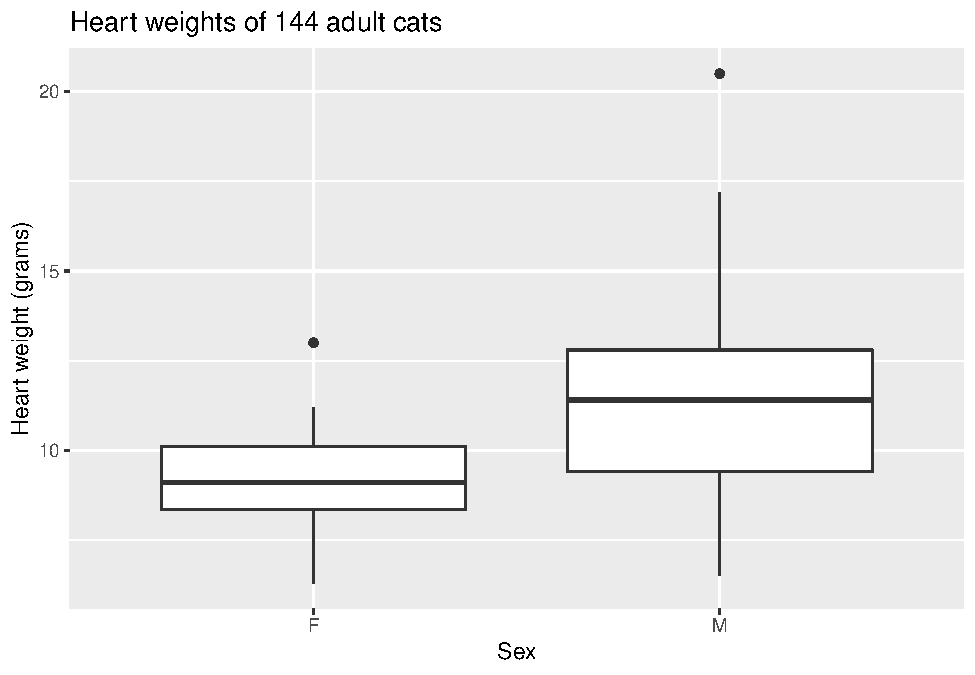
\includegraphics[width=0.68\linewidth]{2561551_PracticeClassTest_files/figure-latex/boxplot-1} 

}

\caption{\label{fig:box} Heart weight by Sex.}\label{fig:boxplot}
\end{figure}

Comment: the boxplot shows that the male cats having heavier hearts, in
general, compared to the female cats' hearts and the weights of the male
hearts were more widely distributed. There are also potentially two
outliers(one male and one female) which have unusually heavy hearts, as
shown by the two points beyond the whiskers of the boxplot.

\hypertarget{sec:FDA}{%
\section{Formal Data Analysis}\label{sec:FDA}}

Comment: To begin to analyse the cat heart weights data formally, we fit
the following linear model to the data.
\[\widehat{\mbox{Hwt}}=\widehat{\alpha}+\widehat{\beta}_{\mbox{Male}}+
\cdot \mathbb{I}_{\mbox{Male}}(x)\]

where

\begin{itemize}
\item
  the intercept \(\widehat{\alpha}\) is the mean heart weight for the
  baseline category of Females;
\item
  \(\widehat{\beta}_{\mbox{Male}}\) is the difference in the mean heart
  weight of a Males relative to the baseline category Females; and
\item
  \(\mathbb{I}_{\mbox{Male}}(x)\) is an indicator function such that
\item
  \[\mathbb{I}_{\mbox{Male}}(x)=\left\{
  \begin{array}{ll}
  1 ~~~ \mbox{if Sex of} ~ x \mbox{th observation is Male},\\
  0 ~~~ \mbox{Otherwise}.\\
  \end{array}
  \right.\]
\end{itemize}

Comment: when this model is fitted to the data, the following estimate
of \(\alpha\)(intercept) and \(\beta_{\mbox{Male}}\)(SexM) are returned:

\begin{table}[H]

\caption{\label{tab:unnamed-chunk-2}\label{tab:reg} Estimates of the parameters from the fitted linear
    regression model.}
\centering
\begin{tabular}[t]{l|r}
\hline
term & estimate\\
\hline
intercept & 9.202\\
\hline
SexM & 2.121\\
\hline
\end{tabular}
\end{table}

Comment: Hence the model estimates the average heart weight of female
cats in 9.202 grams(which agree with the sample mean reported in table
1) and that the male cats' heart weight are, on average, 2.121 grams
heavier than the female cats' heart weights.

Before we can proceed to use the fitted model(for example to perform
statistical inference) we must check the assumptions of the model. These
are best considered in light of the residual plots in Figure 2.

NB: THE DIAGNOSTICS IN THE REMAINDER OF THIS ANALYSIS SECTION ARE NOT
REQUIRED FOR THE CLASS TEST

\begin{figure}[H]

{\centering 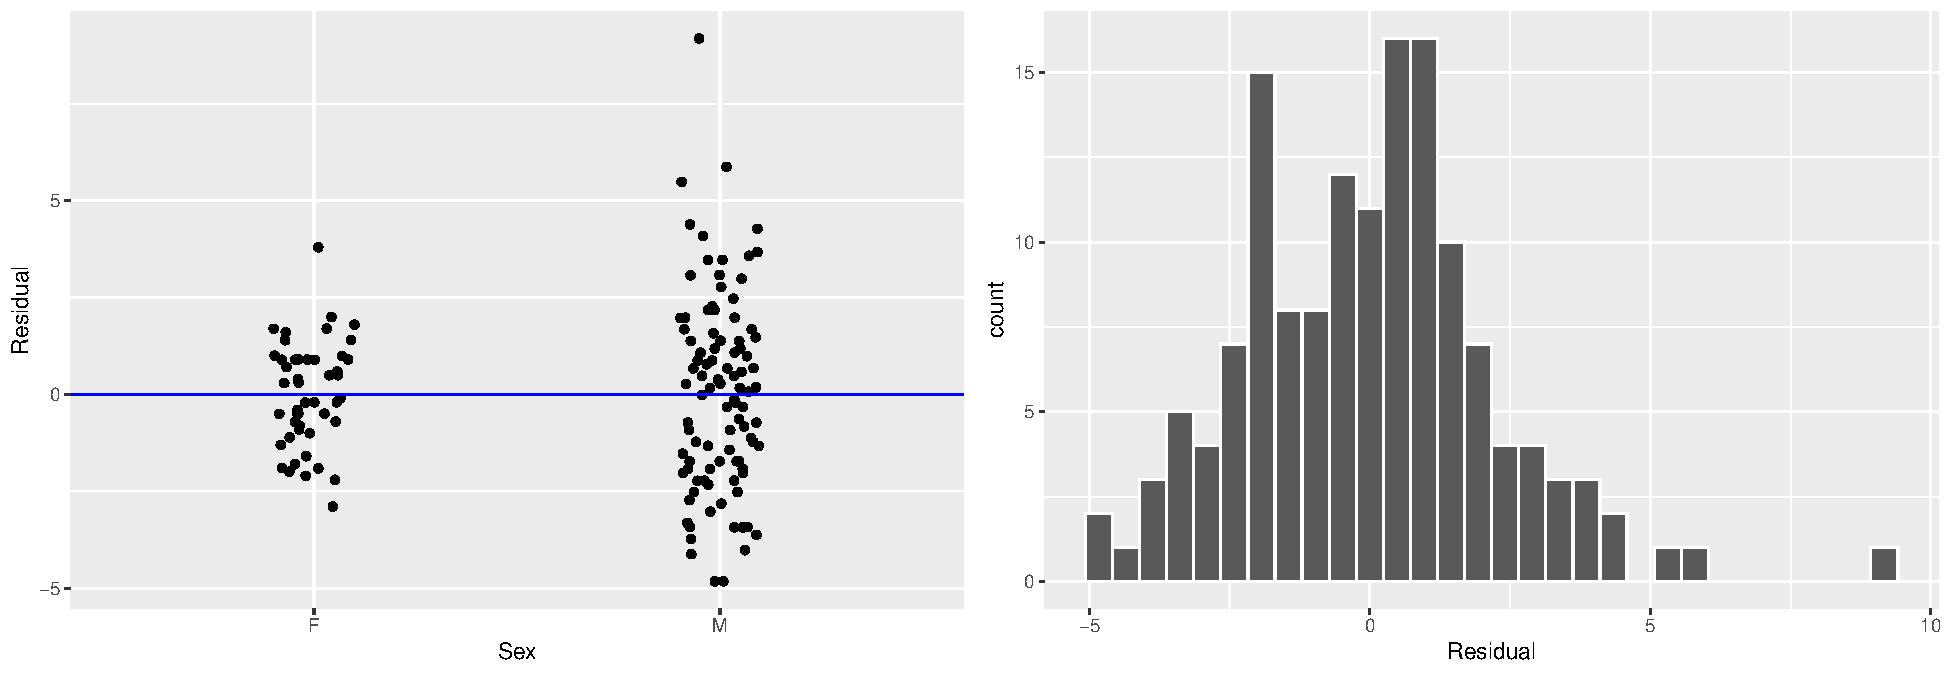
\includegraphics{2561551_PracticeClassTest_files/figure-latex/residplots-1} 

}

\caption{\label{fig:resids} Scatterplots of the residuals by Sex (left) and a histogram of the residuals (right).}\label{fig:residplots}
\end{figure}

In summary, we have estimated that on average, the male cats have hearts
which weight 2.121 grams more than the female cats' hearts. In
particular, we estimate the average heart weight of female cats in 9.202
grams and the average heart weight of male cats is 11.3 grams.

In addition to the centers of distributions of male and female cats'
heart weights being different, we have also observed that the spread of
the male heart weights is greater than the spread of the female cats'
heart weights. This may pose a problem if the standard linear model was
used to further analyse this data, and therefore it is recommended that
models which allow for difference in variance within different group is
used.

\begin{center}\rule{0.5\linewidth}{0.5pt}\end{center}

\newpage

\hypertarget{further-task}{%
\section{FURTHER TASK}\label{further-task}}

\begin{Shaded}
\begin{Highlighting}[]
\KeywordTok{setwd}\NormalTok{(}\StringTok{"/Users/kurisuuu/Documents/glasgow_stats_2021/semester\textbackslash{} 2/das/Practice\textbackslash{} Class\textbackslash{} Test\textbackslash{} Files-20210604"}\NormalTok{)}
\NormalTok{Glasgow_Ed_SIMD2020 <-}\StringTok{ }\KeywordTok{read.csv}\NormalTok{(}\StringTok{"Glasgow_Edinburgh_SIMD2020.csv"}\NormalTok{)}
\end{Highlighting}
\end{Shaded}

The data is not in tidy format since the measurement of interest is rank
which there are 8 types spread over 8 columns.\\
In tidy format the rank measurements should be in a single column, with
a seperate column indicating the type of rank.

To convert the data into a tidy format, use

\begin{Shaded}
\begin{Highlighting}[]
\NormalTok{Glasgow_Ed_SIMD2020_tidy2 <-}\StringTok{ }\KeywordTok{gather}\NormalTok{(}\DataTypeTok{data =}\NormalTok{ Glasgow_Ed_SIMD2020,}
\DataTypeTok{key =}\NormalTok{ Type_of_Rank,}
\DataTypeTok{value =}\NormalTok{ Rank,}
\OperatorTok{-}\NormalTok{(Data_Zone}\OperatorTok{:}\NormalTok{Working_Age_population))}
\NormalTok{Glasgow_Ed_SIMD2020_tidy2}\OperatorTok{$}\NormalTok{Type_of_Rank <-}
\KeywordTok{str_replace}\NormalTok{(Glasgow_Ed_SIMD2020_tidy2}\OperatorTok{$}\NormalTok{Type_of_Rank, }\StringTok{"_Rank"}\NormalTok{, }\StringTok{""}\NormalTok{)}
\end{Highlighting}
\end{Shaded}

\begin{Shaded}
\begin{Highlighting}[]
\NormalTok{Gla_Ed_SIMD2020 <-}\StringTok{ }\NormalTok{Glasgow_Ed_SIMD2020_tidy2 }\OperatorTok
\KeywordTok{filter}\NormalTok{(Type_of_Rank }\OperatorTok{==}\StringTok{ "SIMD"}\NormalTok{) }\OperatorTok\StringTok{ }\CommentTok{#2 MARKS}
\KeywordTok{mutate}\NormalTok{(}\DataTypeTok{Perc_Working =} \DecValTok{100} \OperatorTok{*}\NormalTok{Working_Age_population}\OperatorTok{/}\NormalTok{Total_population)}

\KeywordTok{ggplot}\NormalTok{(Gla_Ed_SIMD2020)}\OperatorTok{+}
\KeywordTok{geom_point}\NormalTok{(}\DataTypeTok{mapping=}\KeywordTok{aes}\NormalTok{(}\DataTypeTok{x=}\NormalTok{Perc_Working,}\DataTypeTok{y=}\NormalTok{Rank,}\DataTypeTok{group=}\NormalTok{Council_area,}\DataTypeTok{color=}\NormalTok{Council_area))}\OperatorTok{+}\StringTok{ }\CommentTok{#3 MARKS}
\KeywordTok{labs}\NormalTok{(}\DataTypeTok{x=}\StringTok{"Employment Rate of Working Age Population"}\NormalTok{,}\DataTypeTok{y=}\StringTok{"SIMD2020 Rank"}\NormalTok{)}
\end{Highlighting}
\end{Shaded}

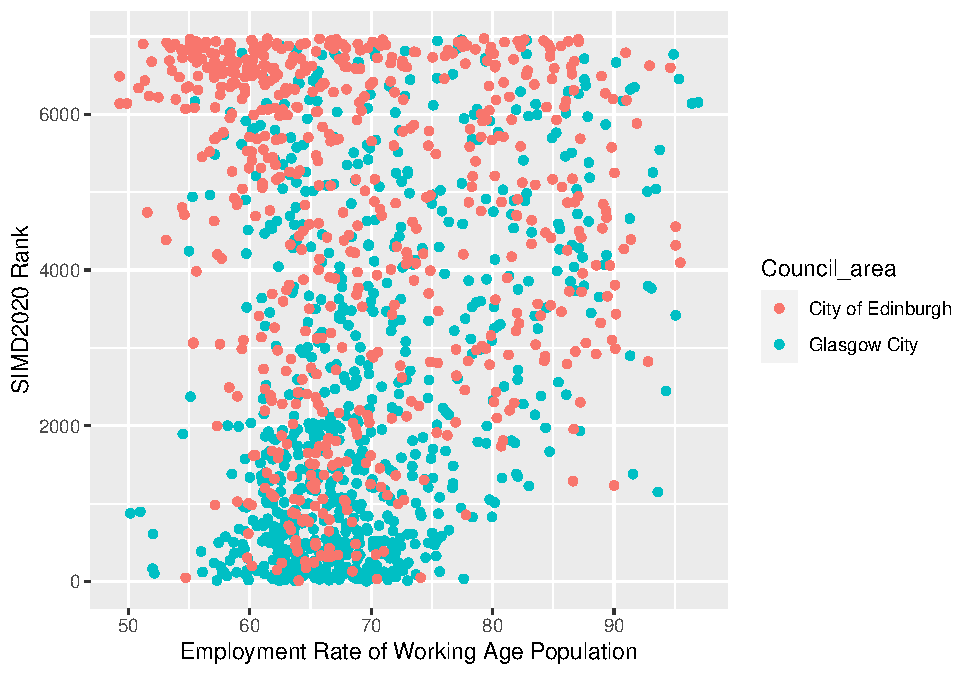
\includegraphics{2561551_PracticeClassTest_files/figure-latex/unnamed-chunk-5-1.pdf}

\end{document}
